%\documentclass[10pt,handout]{beamer}
\documentclass[10pt]{beamer}
\usepackage[ngerman]{babel}
\usepackage[utf8]{inputenc}
\usepackage{amsmath}
\usepackage{amssymb}
\usepackage{listings} 
\usepackage{mathtools}
\usepackage{ulem}
\usepackage{hyperref}
\usetheme{Boadilla}

\parskip 10pt
\lstset{language=Python, tabsize=4, basicstyle=\footnotesize, showstringspaces=false,mathescape=true}  
\lstset{literate=%
  {Ö}{{\"O}}1
  {Ä}{{\"A}}1
  {Ü}{{\"U}}1
  {ß}{{\ss}}1
  {ü}{{\"u}}1
  {ä}{{\"a}}1
  {ö}{{\"o}}1
}
\begin{document}
\title{Codierung ganzer Zahlen}   
\author{Informatik} 
\date{ } 

\frame{\titlepage} 

%-------------
\begin{frame}[fragile]
Information und Daten

\begin{minipage}[c]{6.5cm}
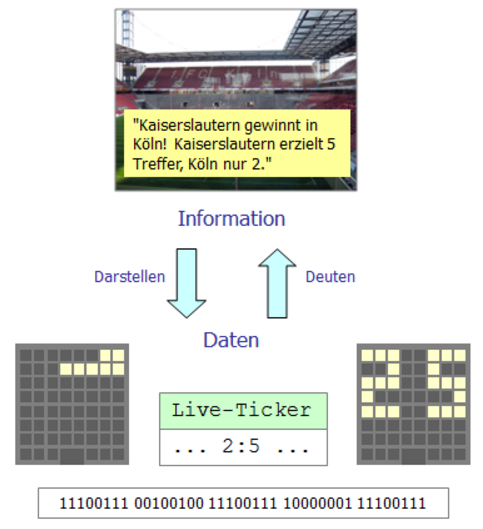
\includegraphics[width=6cm]{bild1.png}
\end{minipage} 
\begin{minipage}[c]{5cm}
\textbf{Information} muss immer in geeigneter Weise dargestellt werden, um sie als \textbf{Daten} maschinell weiterverarbeiten zu können.

Aus Daten gewinnt man erst dann Information, wenn sie gedeutet werden können.
\end{minipage} 
\end{frame}

\begin{frame}[fragile]
Zur Darstellung von Information nutzt man häufig Systeme, die nur zwei Zustände einnehmen können: 
 an/aus; geladen/ungeladen; Strom fließt/Strom fließt nicht; magnetisiert/unmagnetisiert.
 
Ein einfacher Speicher, bei dem Information mit Hilfe (un)geladener Kondensatoren dargestellt wird:

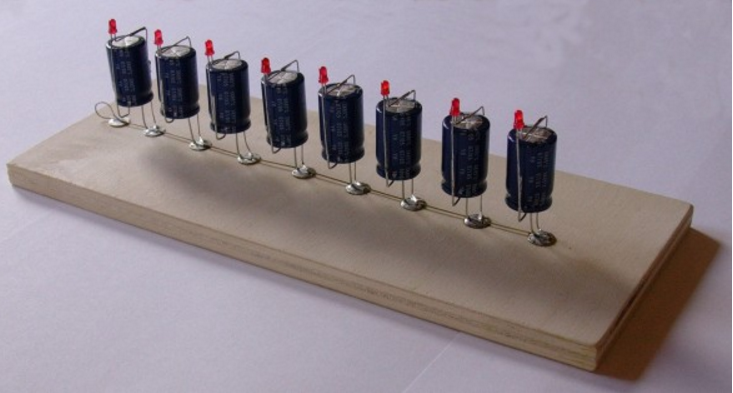
\includegraphics[width=6cm]{bild2.png}

Die beiden Zustände eines Zweizustandssystems werden in der Regel mit Hilfe der beiden Ziffern 0 und 1 beschrieben.
\end{frame}

\begin{frame}[fragile]
Unter einem \textbf{Bit} versteht man eine Einheit zur Informationsdarstellung, die nur zwei Werte annehmen kann: 0 und 1.

Unter einem \textbf{Byte} versteht man eine Einheit aus 8 Bits.  

\begin{tabular}{|l|l|c|}
\hline 1 Byte & 8 Bit  \\
\hline 1 KiloByte (KB) & 1000 Byte \\
\hline 1 Megabyte (MB) & 1000 KB \\
\hline 1 Gigabyte (GB) & 1000 MB \\
\hline 
\end{tabular} \pause

Diese Einheiten bauen auf Zweierpotenzen statt Zehnerpotenzen auf:

\begin{tabular}{|l|l|c|}
\hline 1 KibiByte (KiB) & 1024 Byte \\
\hline 1 Mebibyte (MiB) & 1024 KiB \\
\hline 1 Gibibyte (GiB) & 1024 MiB \\
\hline 
\end{tabular}
\end{frame}

\begin{frame}[fragile]
Ein 16GB USB-Stick im Windows-Explorer:

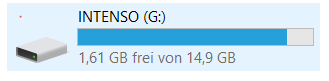
\includegraphics[width=6cm]{bild3.png} \pause

\begin{lstlisting}
# konvertiert gigabyte in gibibyte
def gb2gib(x):
     bytes = 1000 * 1000 * 1000 * x
     return round(bytes / (1024 * 1024 * 1024),2) 
     
>>> gb2gib(16)
14.9
\end{lstlisting} 

Werden die Daten nur mit Bits dargestellt spricht man von
einer \textbf{Binärdarstellung der Daten}. 

Im folgenden geht es um die Binärdarstellung von ganzen Zahlen.
\end{frame}


\begin{frame}[fragile]

\begin{tabbing} Dezimalzahlen~~~~~~~~~ \= 10 Ziffern: $0,1,2, ... 9$ 
~~~~~~~~~~~~~~~~~~~~~~~\=  $4719$  \\   
Dualzahlen \> 2 Ziffern: $0,1$ \>$10010$ \\  
Oktalzahlen \> 8 Ziffern: $0,1,2, ... 7$  \>  $273$ \\  
Hexadezimalzahlen \> 16 Ziffern: $0,1,2, ... 9, A, B, C, D, E, F$ \>$E52F$
 \end{tabbing} \pause

$(4719)_{10} = \pause  9 \cdot 10^0 + 1 \cdot 10^1 + 7 \cdot 10^2 + 4 \cdot 10^3$ \\  
$(273)_{8} = \pause 3 \cdot 8^0 + 7 \cdot 8^1 + 2 \cdot 8^2 = (187)_{10}$\\  
$(10010)_{2} =  \pause 0 \cdot 2^0 + 1 \cdot 2^1 + 0 \cdot 2^2 + 0 \cdot 2^3 + 1 \cdot 2^4 = (18)_{10}$ \\  
$(E52F)_{16} = \pause 15 \cdot 16^0 + 2 \cdot 16^1 + 5 \cdot 16^2 + 14 \cdot 16^3 = (58671)_{10}$

\end{frame}

\begin{frame}[fragile]
Umwandlung Dualzahl in Dezimalzahl

\begin{lstlisting}[mathescape=true]
def dual_dez(s):  
    '''
    s: String aus 0 und 1
    returns: Dezimalzahl, die der Dualzahl s entspicht
    '''  $\pause$
    x = 0
    sw = 1   # Stellenwert
    for c in s[::-1]:
        if c $==$ '1':
            x+=sw
        sw*=2
    return x
\end{lstlisting} 

Aufruf: 
\begin{lstlisting}
>>> dual_dez('1101')
13  
\end{lstlisting} 
\end{frame}

\begin{frame}[fragile]
$10110 / 2   =  ( 1 \cdot 2^4 +  0 \cdot 2^3 + 1 \cdot 2^2 + 1 \cdot 2^1 + 0 \cdot 2^0 ) / 2 = $\\ 
~~~~~~~~~~~~~~~$(1 \cdot 2^3 + 0 \cdot 2^2 + 1 \cdot 2^1 + 1 \cdot 2^0 ) = 1011$ \pause

ganzzahlige Division durch 2: \pause  die rechte Ziffer verschwindet \\
Multiplikation mit 2: \pause rechts kommt noch eine 0 dran. 


\begin{tabbing}
10110 ~~~~ \= 22 \\
1011  \pause \> 11 \\
101 \pause \> 5 \\
10  \pause \> 2 \\
101100  \pause \> 44
 \end{tabbing}

\end{frame}

\begin{frame}[fragile]
Umrechnung von 13 in eine Dualzahl   
\begin{tabbing}


xxxx ~~~~ \= 13 ~~~~~~~~~~~ \pause \= ~~~~\= 1 \\
xxx \> $6$ \>  \> 0 \\
xx \> $3$ \>  \> 1 \\
x \> $1$ \>  \> 1 \\
\> $0$ \>  
 \end{tabbing}
Dualzahl ergibt sich von unten nach oben: 1101
\end{frame}

\begin{frame}[fragile]
Unsere Schreibweise zur Umrechnung:
\vspace{-0.3cm}
\begin{tabbing}
13 ~~ \=  \\
6 \> 1 \\
3 \> 0 \\
1 \> 1 \\
0 \> 1 
 \end{tabbing}
\vspace{-0.3cm}
Dezimalzahl 13 ist Dualzahl 1101  

\vspace{-0.3cm}
\begin{tabbing}
41 ~~ \=  \\ \pause
20 \> 1 \\
10 \> 0 \\
5 \> 0 \\
2\> 1 \\
1 \> 0 \\ 
0 \> 1
 \end{tabbing}
\vspace{-0.3cm}
Dezimalzahl 41 ist Dualzahl 101001 
\end{frame}

%------
\begin{frame}[fragile]
Umrechnung einer Dezimalzahl in eine Oktalzahl
\vspace{-0.3cm}
\begin{tabbing}
41 ~~ \pause  \=  \\
5 \> 1 \\
0 \> 5
 \end{tabbing}
\vspace{-0.3cm}
Dezimalzahl 41 ist Oktalzahl 51 \pause

Umrechnung einer Dezimalzahl in eine Hexadezimalzahl
\begin{tabbing}
3882 ~~  \pause \=  \\
242 \> A \\
15 \> 2 \\
0\> F
 \end{tabbing}
\vspace{-0.3cm}
Dezimalzahl 3882 ist Hexadezimalzahl F2A 
\end{frame}
%---

\begin{frame}[fragile]
Umrechnung Dezimalzahl in Dualzahl 
\begin{lstlisting}
def dez_dual(x): $\pause$
    if x $==$ 0: return '0'
    s = ""                 
    while x != 0:
        s = str(x%2) + s
        x = x // 2
    return s
\end{lstlisting}

Aufruf:
\begin{lstlisting}
>>> dez_dual(47)
'101111'    


\end{lstlisting} 
\end{frame}

\begin{frame}[fragile]
Die Addition von Dualzahlen erfolgt analog zum Dezimalsystem. Die Stellenwerte werden addiert, gegebenenfalls mit Übertrag.

\begin{tabbing}
 ~~~~ \= 0 ~~~ \= 1 ~~~ \= 0 ~~~ \= 1 ~~~\= 0 \\
+ \>1 \> 1 \> 0 \> 1 \> 1 \\
\\ \pause
1 \>0 \> 0 \> 1 \> 0 \> 1 \\
 \end{tabbing} 


\end{frame}


\begin{frame}[fragile]
Mit 3 bit können die Zahlen von 0-7 dargestellt werden
\begin{tabbing}
1 ~~~ \= 1 ~~~ \= 1 ~~~~~~~~~~\= 7 \\
1 \> 1 \> 0 \> 6 \\
1 \> 0 \> 1 \> 5 \\
1 \> 0 \> 0 \> 4 \\
0 \> 1 \> 1 \> 3 \\
0 \> 1 \> 0 \> 2 \\
0 \> 0 \> 1 \> 1 \\
0 \> 0 \> 0 \> 0 
 \end{tabbing}  
Wie kann man negative Zahlen darstellen ?
\end{frame}

\begin{frame}[fragile]

\begin{tabbing}
0 ~~~ \=1 ~~~ \= 1 ~~~ \= 1 ~~~~~~~~~~\= 7 \\
0 \> 1 \> 1 \> 0 \> 6 \\
0 \> 1 \> 0 \> 1 \> 5 \\
0 \> 1 \> 0 \> 0 \> 4 \\
0 \> 0 \> 1 \> 1 \> 3 \\
0 \> 0 \> 1 \> 0 \> 2 \\
0 \> 0 \> 0 \> 1 \> 1 \\
0 \> 0 \> 0 \> 0 \> 0 
 \end{tabbing}
\vspace{-0.5cm}
\begin{tabbing}
1 ~~~ \=1 ~~~ \= 1 ~~~ \= 1 ~~~~~~~~~~\= -7 \\
1 \> 1 \> 1 \> 0 \> -6 \\
1 \> 1 \> 0 \> 1 \> -5 \\
1 \> 1 \> 0 \> 0 \> -4 \\
1 \> 0 \> 1 \> 1 \> -3 \\
1 \> 0 \> 1 \> 0 \> -2 \\
1 \> 0 \> 0 \> 1 \> -1 \\
1 \> 0 \> 0 \> 0 \> -0 
 \end{tabbing}
\textbf{SO NICHT}
\end{frame}

\begin{frame}[fragile]
\begin{tabbing}
0 ~~~ \=1 ~~~ \= 1 ~~~ \= 1 ~~~~~~~~~~\= 7 \\
0 \> 1 \> 1 \> 0 \> 6 \\
0 \> 1 \> 0 \> 1 \> 5 \\
0 \> 1 \> 0 \> 0 \> 4 \\
0 \> 0 \> 1 \> 1 \> 3 \\
0 \> 0 \> 1 \> 0 \> 2 \\
0 \> 0 \> 0 \> 1 \> 1 \\
0 \> 0 \> 0 \> 0 \> 0  \\
\\
1 \> 1 \> 1 \> 1  \> -1  \\
1 \> 1 \> 1 \> 0 \> -2 \\
1 \> 1 \> 0 \> 1 \> -3 \\
1 \> 1 \> 0 \> 0 \> -4 \\
1 \> 0 \> 1 \> 1 \> -5 \\
1 \> 0 \> 1 \> 0 \> -6 \\
1 \> 0 \> 0 \> 1 \> -7 \\
1 \> 0 \> 0 \> 0 \> -8 
 \end{tabbing}
\vspace{-0.5cm}
Die 4-bit Zweierkomplement Darstellung von  $-8 =  -2^3$ bis $7 =  2^3-1$. 


\end{frame}

\begin{frame}[fragile]
Wertebereiche:

\begin{tabular}{|c|c|c|c|c|}
\hline  & Dualzahl & Zweierkomplement \\
\hline 4-Bit &   &   \\
\hline 8-Bit &  &    \\
\hline
\end{tabular}  

Einige Binärdarstellungen im Zweierkomplement: 

\begin{tabular}{|c|c|c|c|c|}
\hline  & 4-Bit & 8-Bit \\
\hline größte Zahl & ~~~~ & ~~~~~~~~~~~~   \\
\hline kleinste Zahl &  &    \\
\hline 1 &  &     \\
\hline -1 &  &     \\
\hline
\end{tabular}
\end{frame}


\begin{frame}[fragile]
Wertebereiche:

\begin{tabular}{|c|c|c|c|c|}
\hline  & Dualzahl & Zweierkomplement \\
\hline 4-Bit & 0 ... 15 & -8 ... +7   \\
\hline 8-Bit & 0 ... 255 & -128 ... +127   \\
\hline
\end{tabular} 

Einige Binärdarstellungen im Zweierkomplement: 

\begin{tabular}{|c|c|c|c|c|}
\hline  & 4-Bit & 8-Bit \\
\hline größte Zahl & 0111 & 0111 1111   \\
\hline kleinste Zahl & 1000 & 1000 0000   \\
\hline 1 & 0001 & 0000 0001   \\
\hline -1 & 1111 & 1111 1111   \\
\hline
\end{tabular}
\end{frame}

\begin{frame}[fragile]
Im Zweierkomplement kann für Addition und Subtraktion derselbe Algorithmus verwendet werden.

%Die 8-bit Zweierkomplement Darstellung geht von  $-2^7$ bis $ 2^7-1$, \\ 
%d.h. von -128 bis 127. \pause

%\begin{tabbing}
%-128 ~~~ \= \pause 1000 0000 \\ \pause
%-1 \> \pause 1111 1111 \\ \pause
%127 \pause \> 0111 1111
% \end{tabbing} \pause

Codierung von -x:
\begin{lstlisting}[mathescape=true]
codiere x
negiere bitweise
addiere 1
\end{lstlisting} \pause

\begin{minipage}[c]{5.5cm}
Codierung von -5 (4 bit) \pause
%\vspace{-0.5cm}
\begin{tabbing}
5  ~~~~~~~~~~~~~~~~~~~~~~~ \= 0101  \\
bitweise Negation  \>  1010\\
addiere 1 \> 0001 \\
-5 \> 1011 
 \end{tabbing} 
\end{minipage} \pause
\begin{minipage}[c]{5.5cm}
 Codierung von -100 (8 bit) \pause
\begin{tabbing}
100  ~~~~~~~~~~~~~~~~~~~~~~~ \= 01100100 \\
bitweise Negation  \> 10011011 \\
addiere 1 \> 00000001 \\
-100 \> 10011100
 \end{tabbing}
 \end{minipage}  
 
Wenn die Verknüpfung die zulässigen Wertebereiche verlässt, entstehen falsche Ergebnisse.
\end{frame}

\begin{frame}[fragile]
In der Programmiersprache Java werden ganze Zahlen vom Typ \texttt{int} intern im 32-bit Zweierkomplement gespeichert.

Was macht dieses Programm?
\begin{lstlisting}[mathescape=true]
	  int k = 1;
	  while (k > 0) 
	    k = k+1;
	  System.out.println(k); $\pause$
	  
-2147483648  	  
\end{lstlisting} \pause

$-2147483648  = -2^{31}$
\end{frame}

\begin{frame}[fragile]
Darstellung des Zweierkomplements im Zahlenkreis:

\begin{minipage}[c]{8cm}
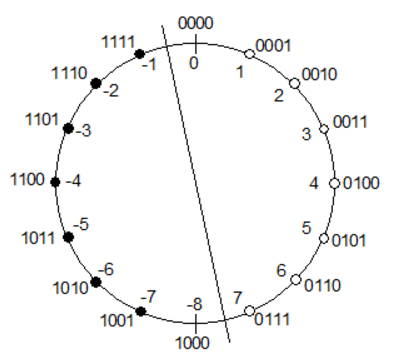
\includegraphics[width=7cm]{bild4.png} 
\end{minipage} \pause
\begin{minipage}[b]{3cm}
\begin{lstlisting}[mathescape=true]
>>> bin(16-5)
'0b1011'
>>> bin(256-100)
'0b10011100'
>>> 

\end{lstlisting} 
\end{minipage} 
\end{frame}
%\begin{frame}[fragile]
%\begin{tabbing}
%~~~~\=3 ~~~~~~~~~~~ \= 0011 \\
%+ \> 2  \> 0010 \\
%=\> 5 \> 0101 \\
% \end{tabbing} \pause
%
%\vspace{-0.5cm}
%\begin{tabbing}
%~~~~\=2 ~~~~~~~~~~~ \= 0010 \\
%- \> 5  \> 1011 \\
%=\> -3 \> 1101 \\
% \end{tabbing} \pause
%
%
%\vspace{-0.5cm}
%\begin{tabbing}
%~~~~\=2 ~~~~~~~~~~~ \= 0010 \\
%+ \> 6  \> 0110 \\
%=\> -8 \> 1000 ~~~~ falsch!\\
% \end{tabbing} \pause
%
%\vspace{-0.5cm}
%Wenn die Verknüpfung die zulässigen Wertebereiche verlässt, entstehen falsche Ergebnisse.
%\end{frame}



%\begin{frame}[fragile]
%Bitweise Operationen in Python
%\begin{lstlisting}
%00111100       60
%00001101       13
%------------------------------
%00001100       12 = 60 & 13
%00111101       61 = 60 | 13
%00110001       49 = 60 ^ 13
%00011110       30 = 60 >> 1
%01111000      120 = 60 << 1
%11000011      195 = 255 - 60
%\end{lstlisting}  \pause
%
%Was erscheint auf der Konsole?
%\begin{lstlisting}
%a, b = 15, 22
%b &= a
%a ^= b
%print(a << 2)
%\end{lstlisting}  \pause
%36
%\end{frame}
 \end{document}
